\subsection{Tutor Pages}

\noindent The tutor interface enables instructors to manage their teaching schedules, sessions, and student progress.

\subsubsection{Tutor Dashboard}

\noindent The tutor dashboard serves as the central hub for instructors, providing a comprehensive overview of their teaching activities, upcoming sessions, student progress, and notifications.

\begin{figure}[H]
    \centering
    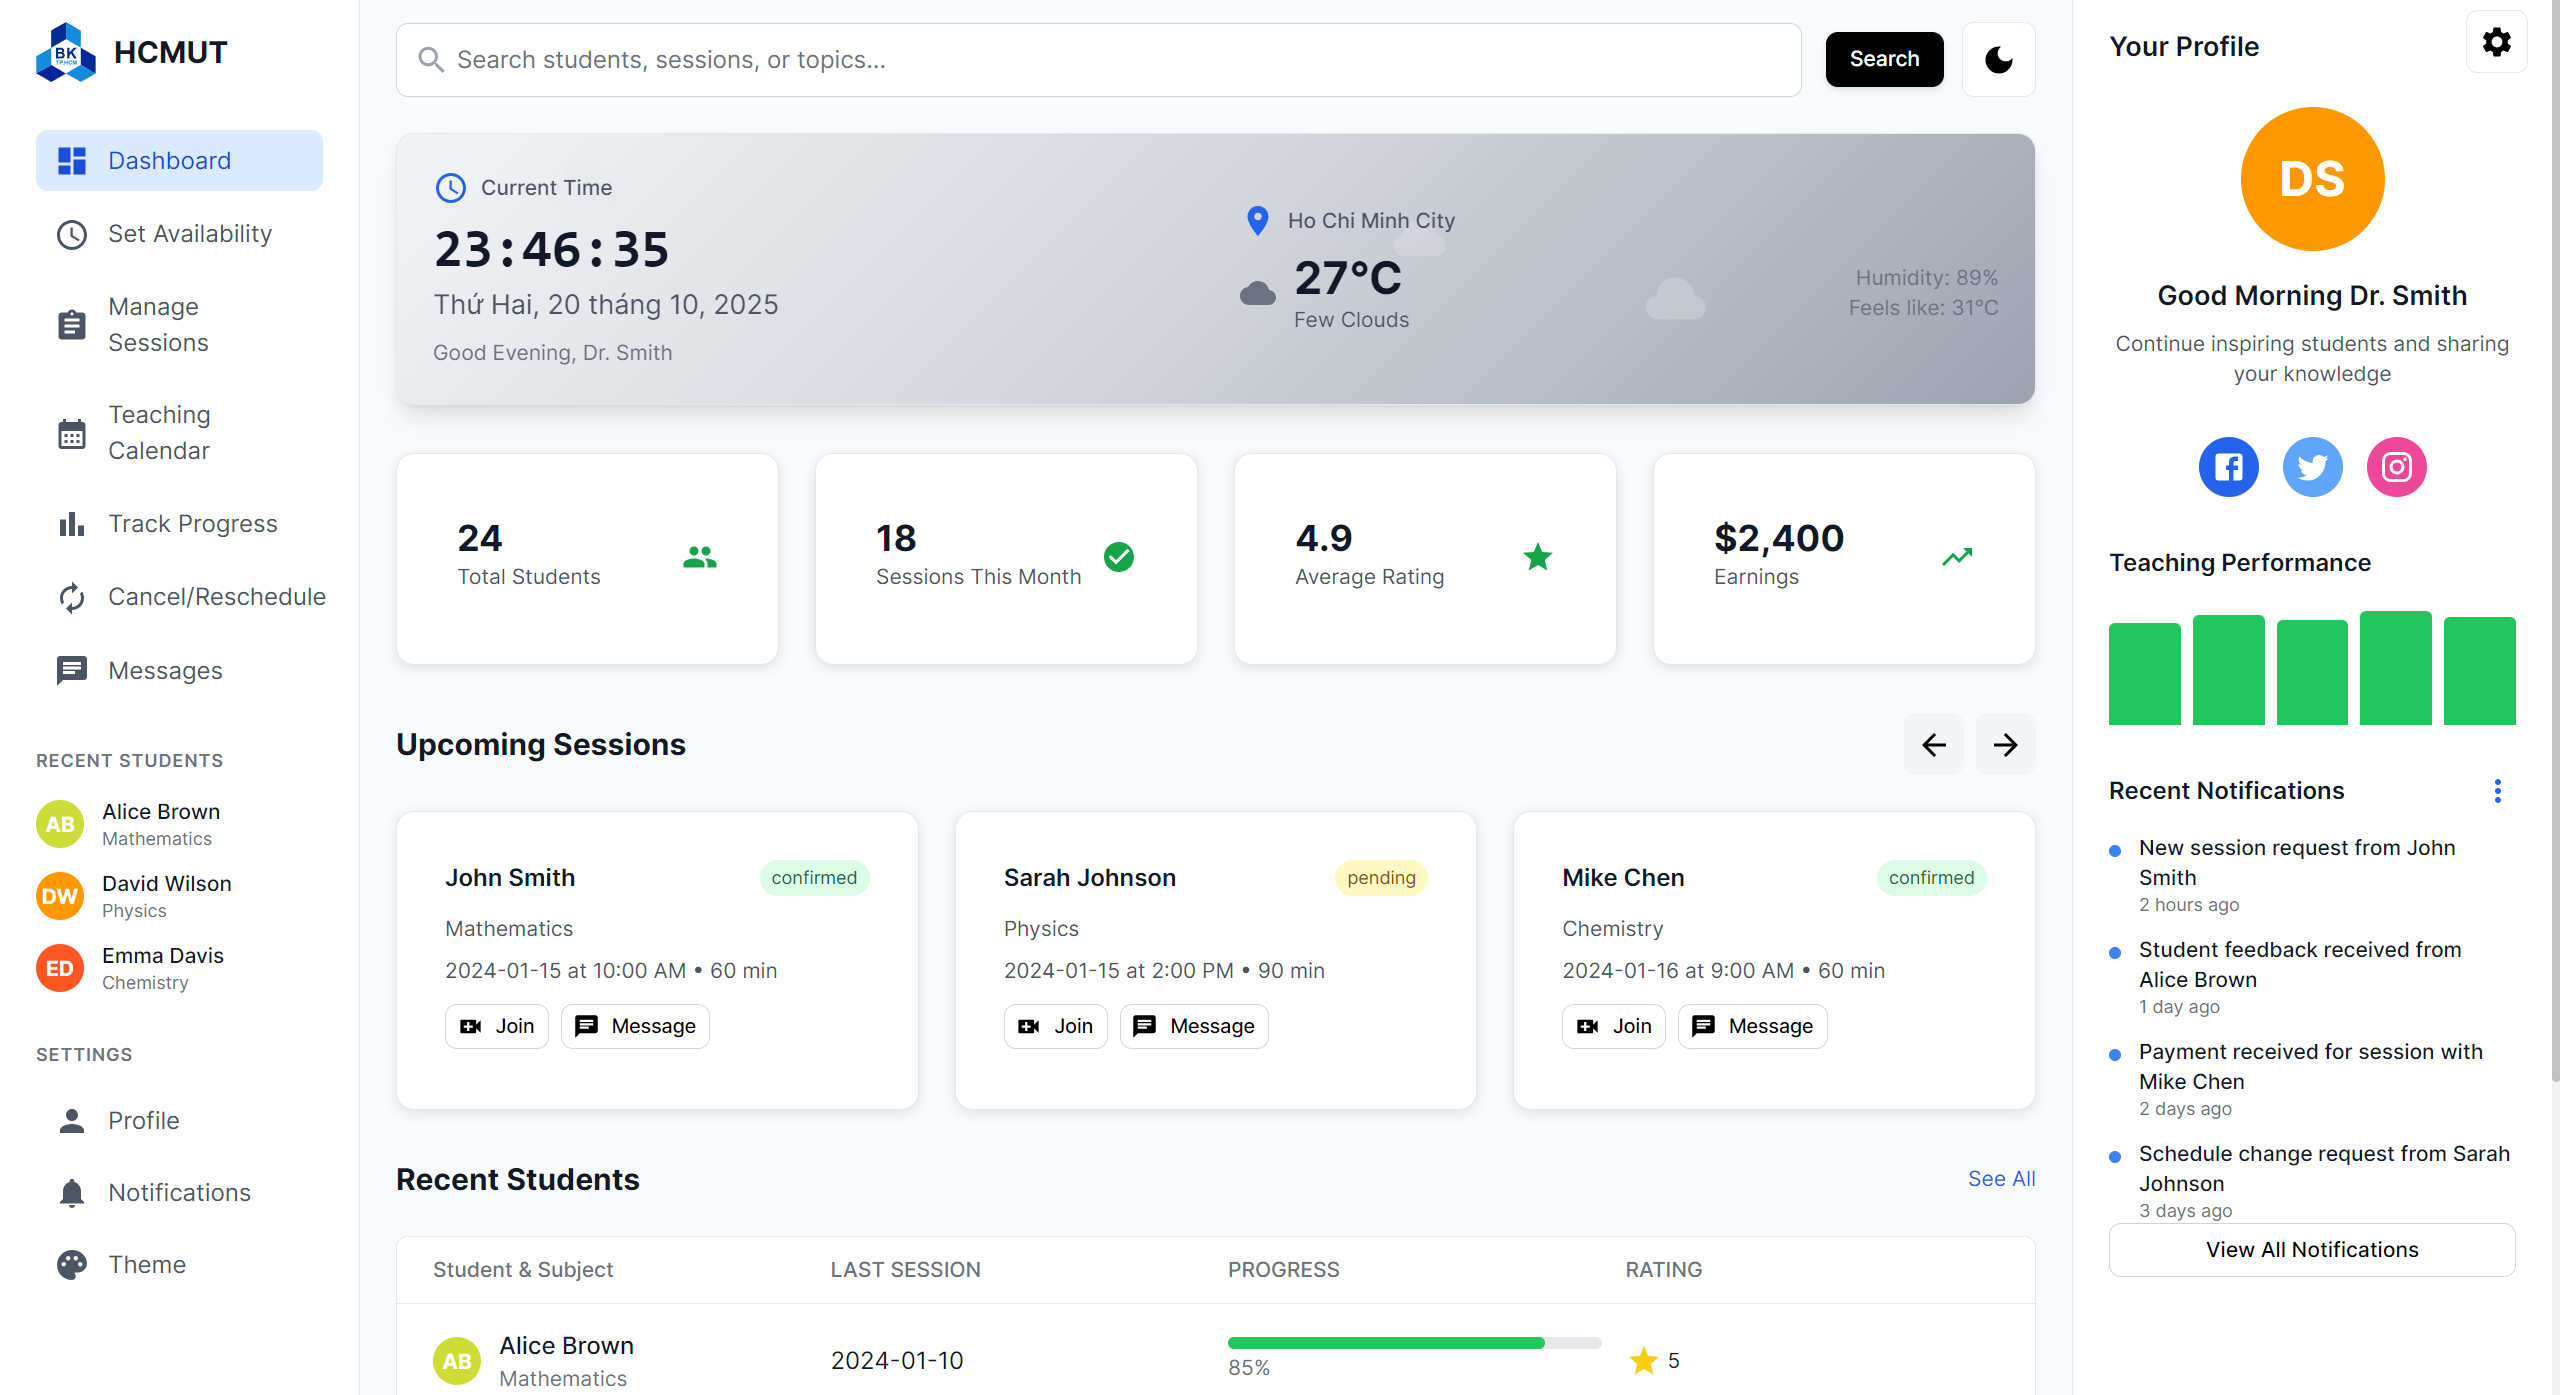
\includegraphics[width=\textwidth]{graphics/chapter2/tutor/tutor_dashboard_overall.png}
    \caption{Tutor Dashboard Overview}
    \label{fig:tutor_dashboard_overall}
\end{figure}

\paragraph{General Overview}
The dashboard features a three-column layout: left navigation sidebar, central content area, and right profile panel.

\subsubsection{Set Availability}

\noindent The "Set Availability" page allows tutors to define and manage their teaching schedule and availability.

\begin{figure}[H]
    \centering
    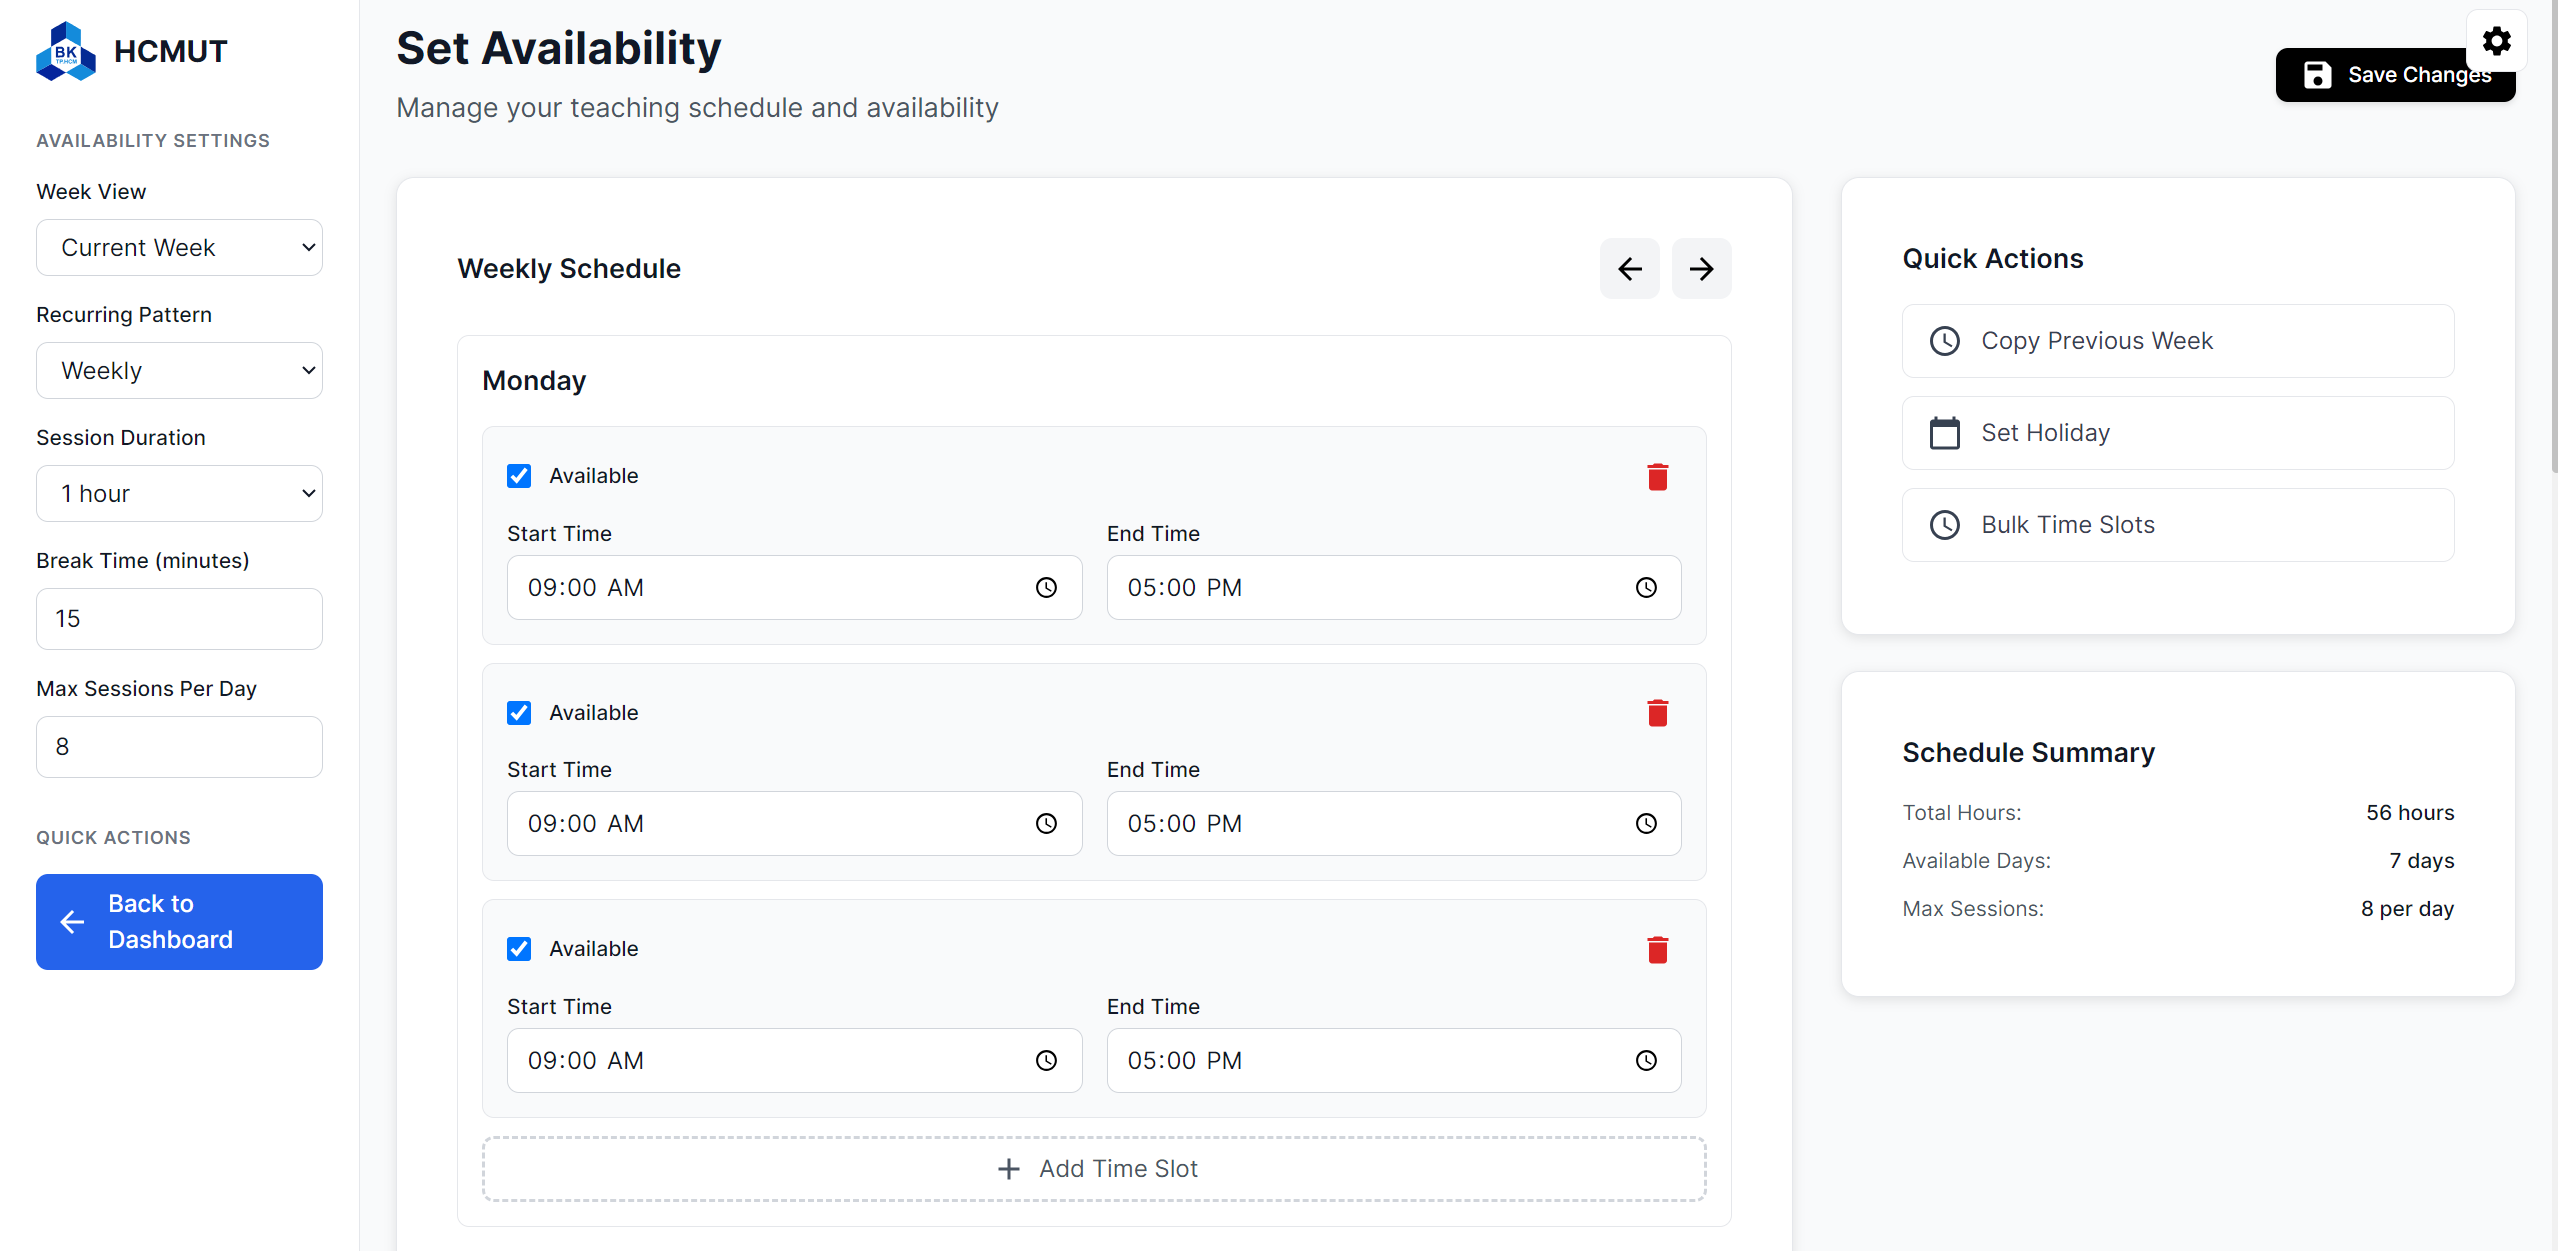
\includegraphics[width=\textwidth]{graphics/chapter2/tutor/set_availability_overall.png}
    \caption{Set Availability Page Overview}
    \label{fig:set_availability_overall}
\end{figure}

\paragraph{General Overview}
The page is structured into three main columns: left sidebar for availability settings, central area for weekly schedule, and right sidebar for quick actions and schedule summary.

\subsubsection{Manage Sessions}

\noindent The "Manage Sessions" page provides tutors with a comprehensive interface to view, filter, and modify all their scheduled teaching sessions.

\begin{figure}[H]
    \centering
    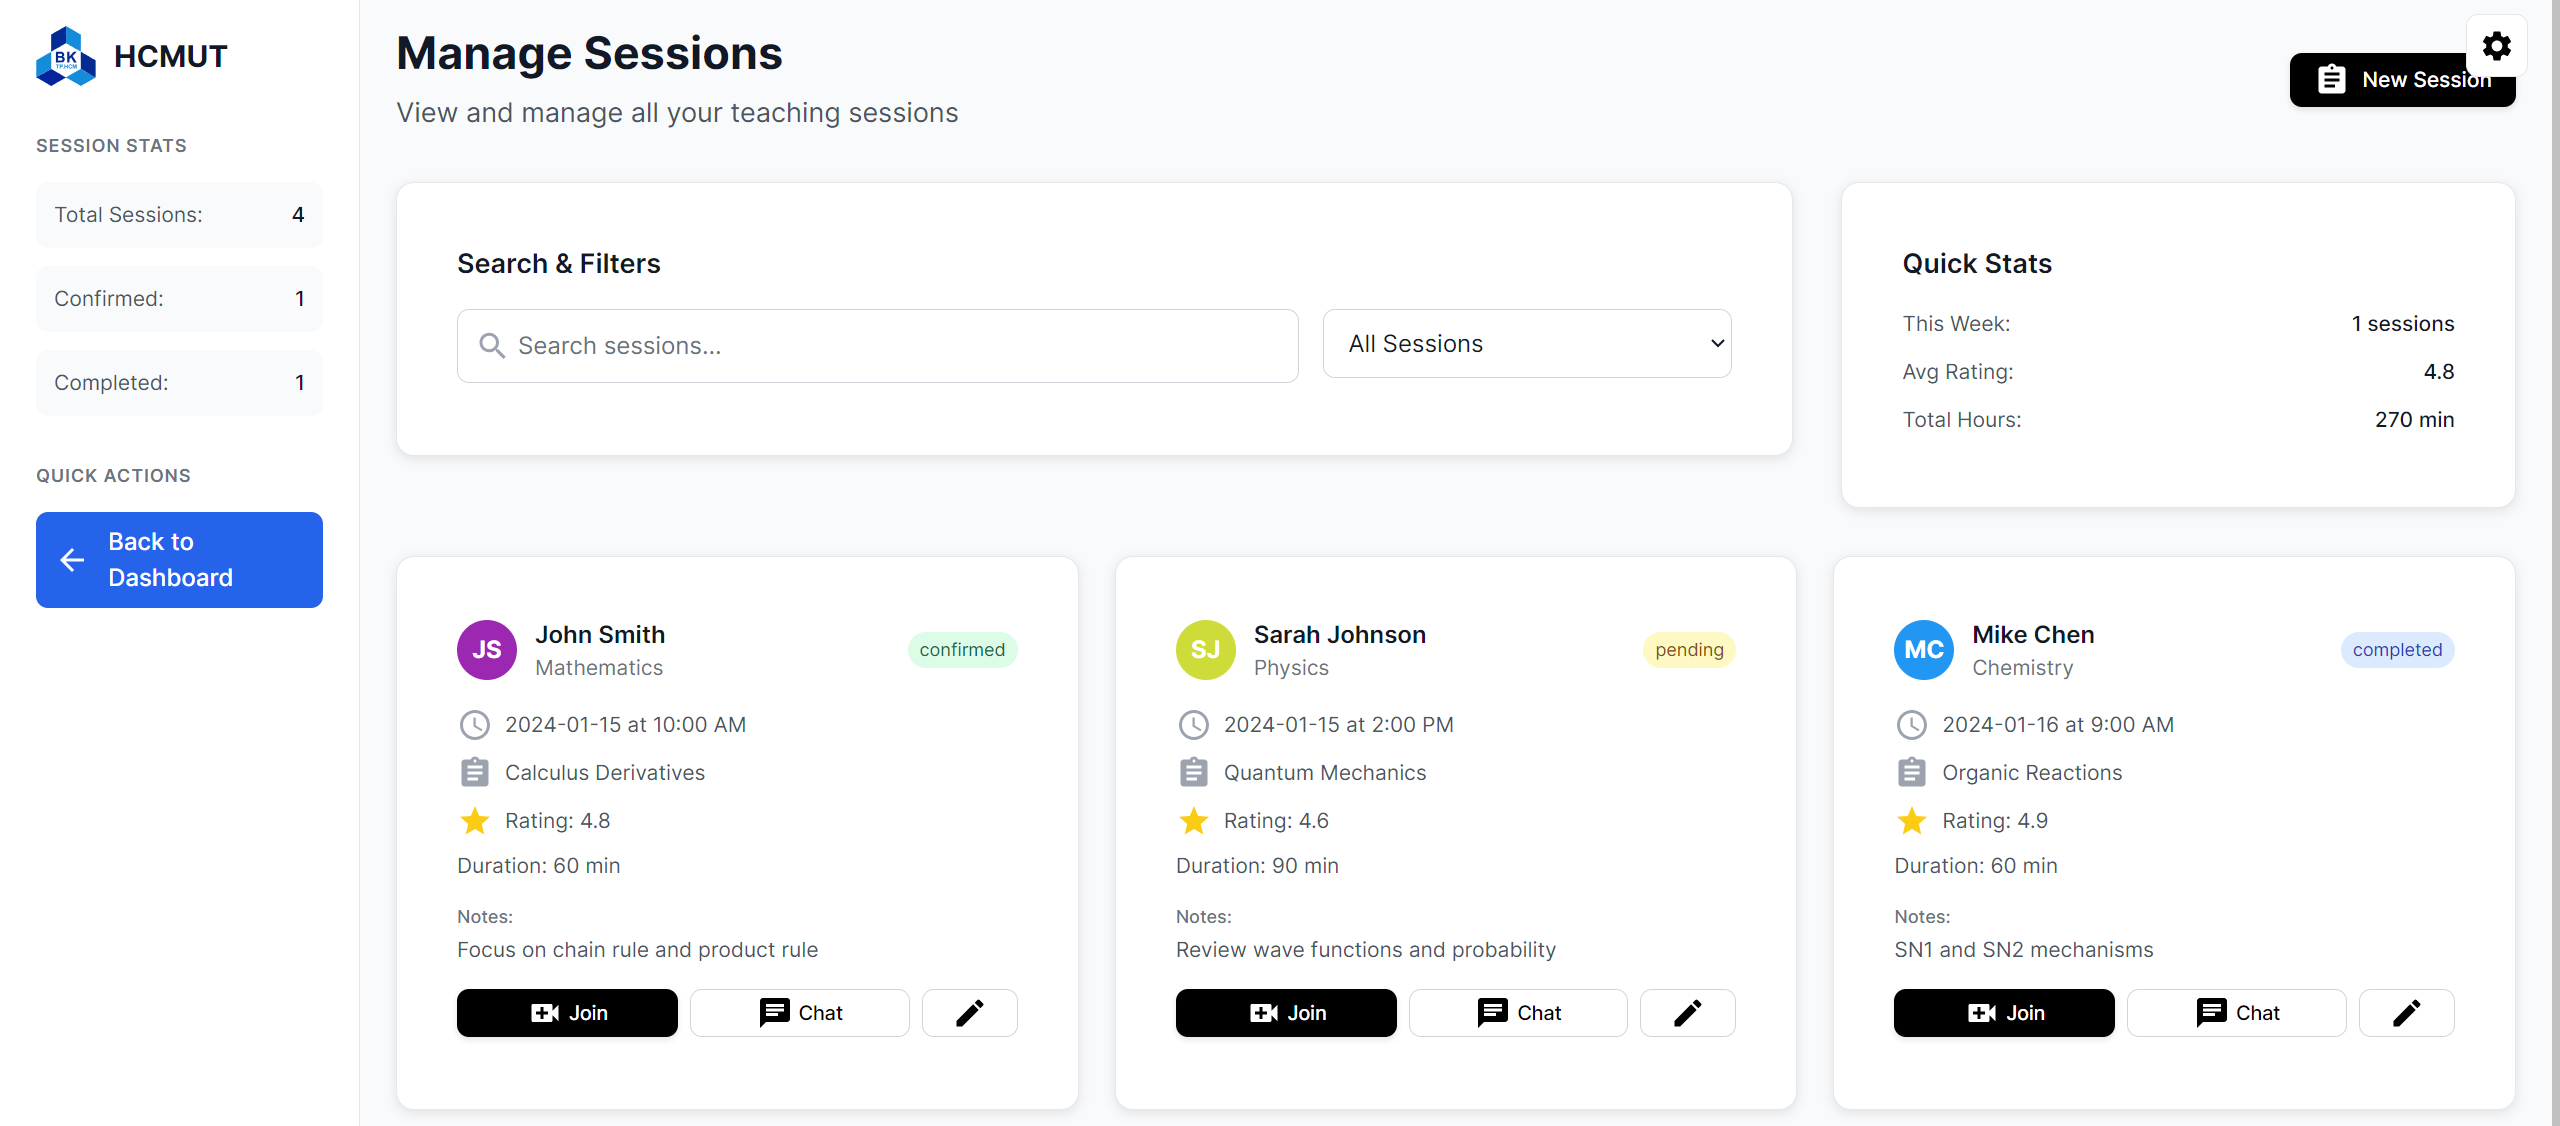
\includegraphics[width=\textwidth]{graphics/chapter2/tutor/manage_sessions_overall.png}
    \caption{Manage Sessions Page Overview}
    \label{fig:manage_sessions_overall}
\end{figure}

\paragraph{General Overview}
The page maintains a three-column layout with session statistics, search and filter options, and individual session cards.

\subsubsection{Cancel / Reschedule}

\noindent The "Cancel / Reschedule Requests" page provides tutors with a dedicated interface to manage student-initiated requests for session cancellations or rescheduling.

\begin{figure}[H]
    \centering
    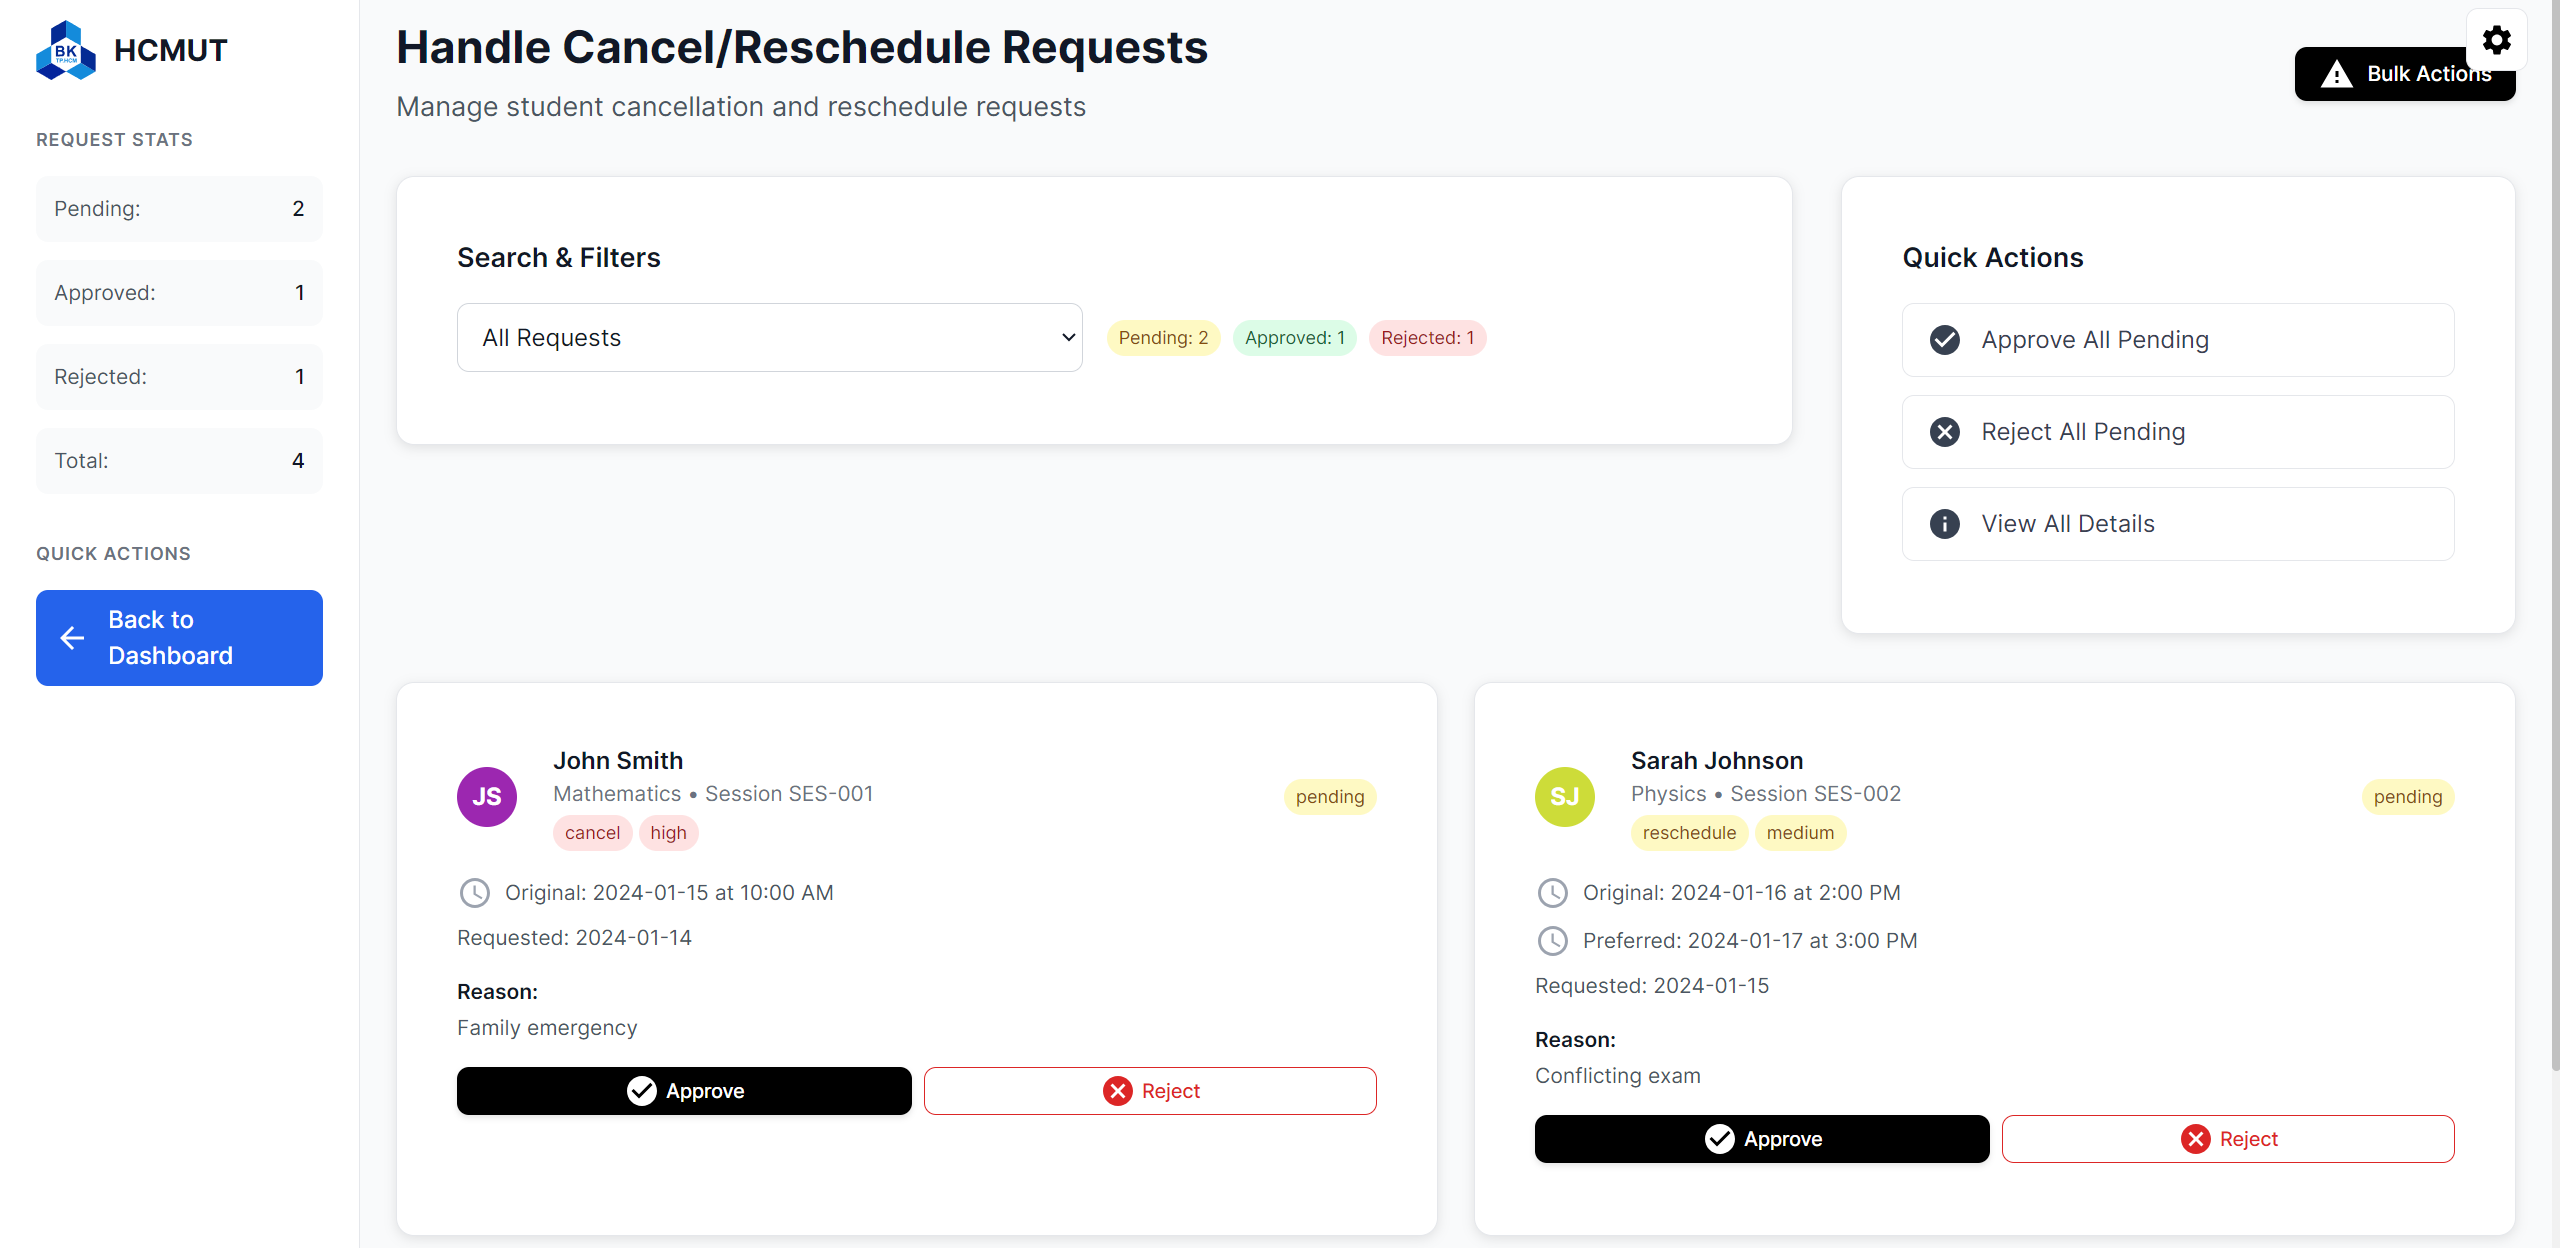
\includegraphics[width=\textwidth]{graphics/chapter2/tutor/cancel_reschedule_overall.png}
    \caption{Cancel / Reschedule Requests Page Overview}
    \label{fig:cancel_reschedule_overall}
\end{figure}

\paragraph{General Overview}
The page maintains a three-column layout with request statistics, search and filter options, and individual request cards.

\subsubsection{Track Student Progress}

\noindent The "Track Student Progress" page provides tutors with a comprehensive overview of their students' academic performance, learning goals, strengths, and areas for improvement.

\begin{figure}[H]
    \centering
    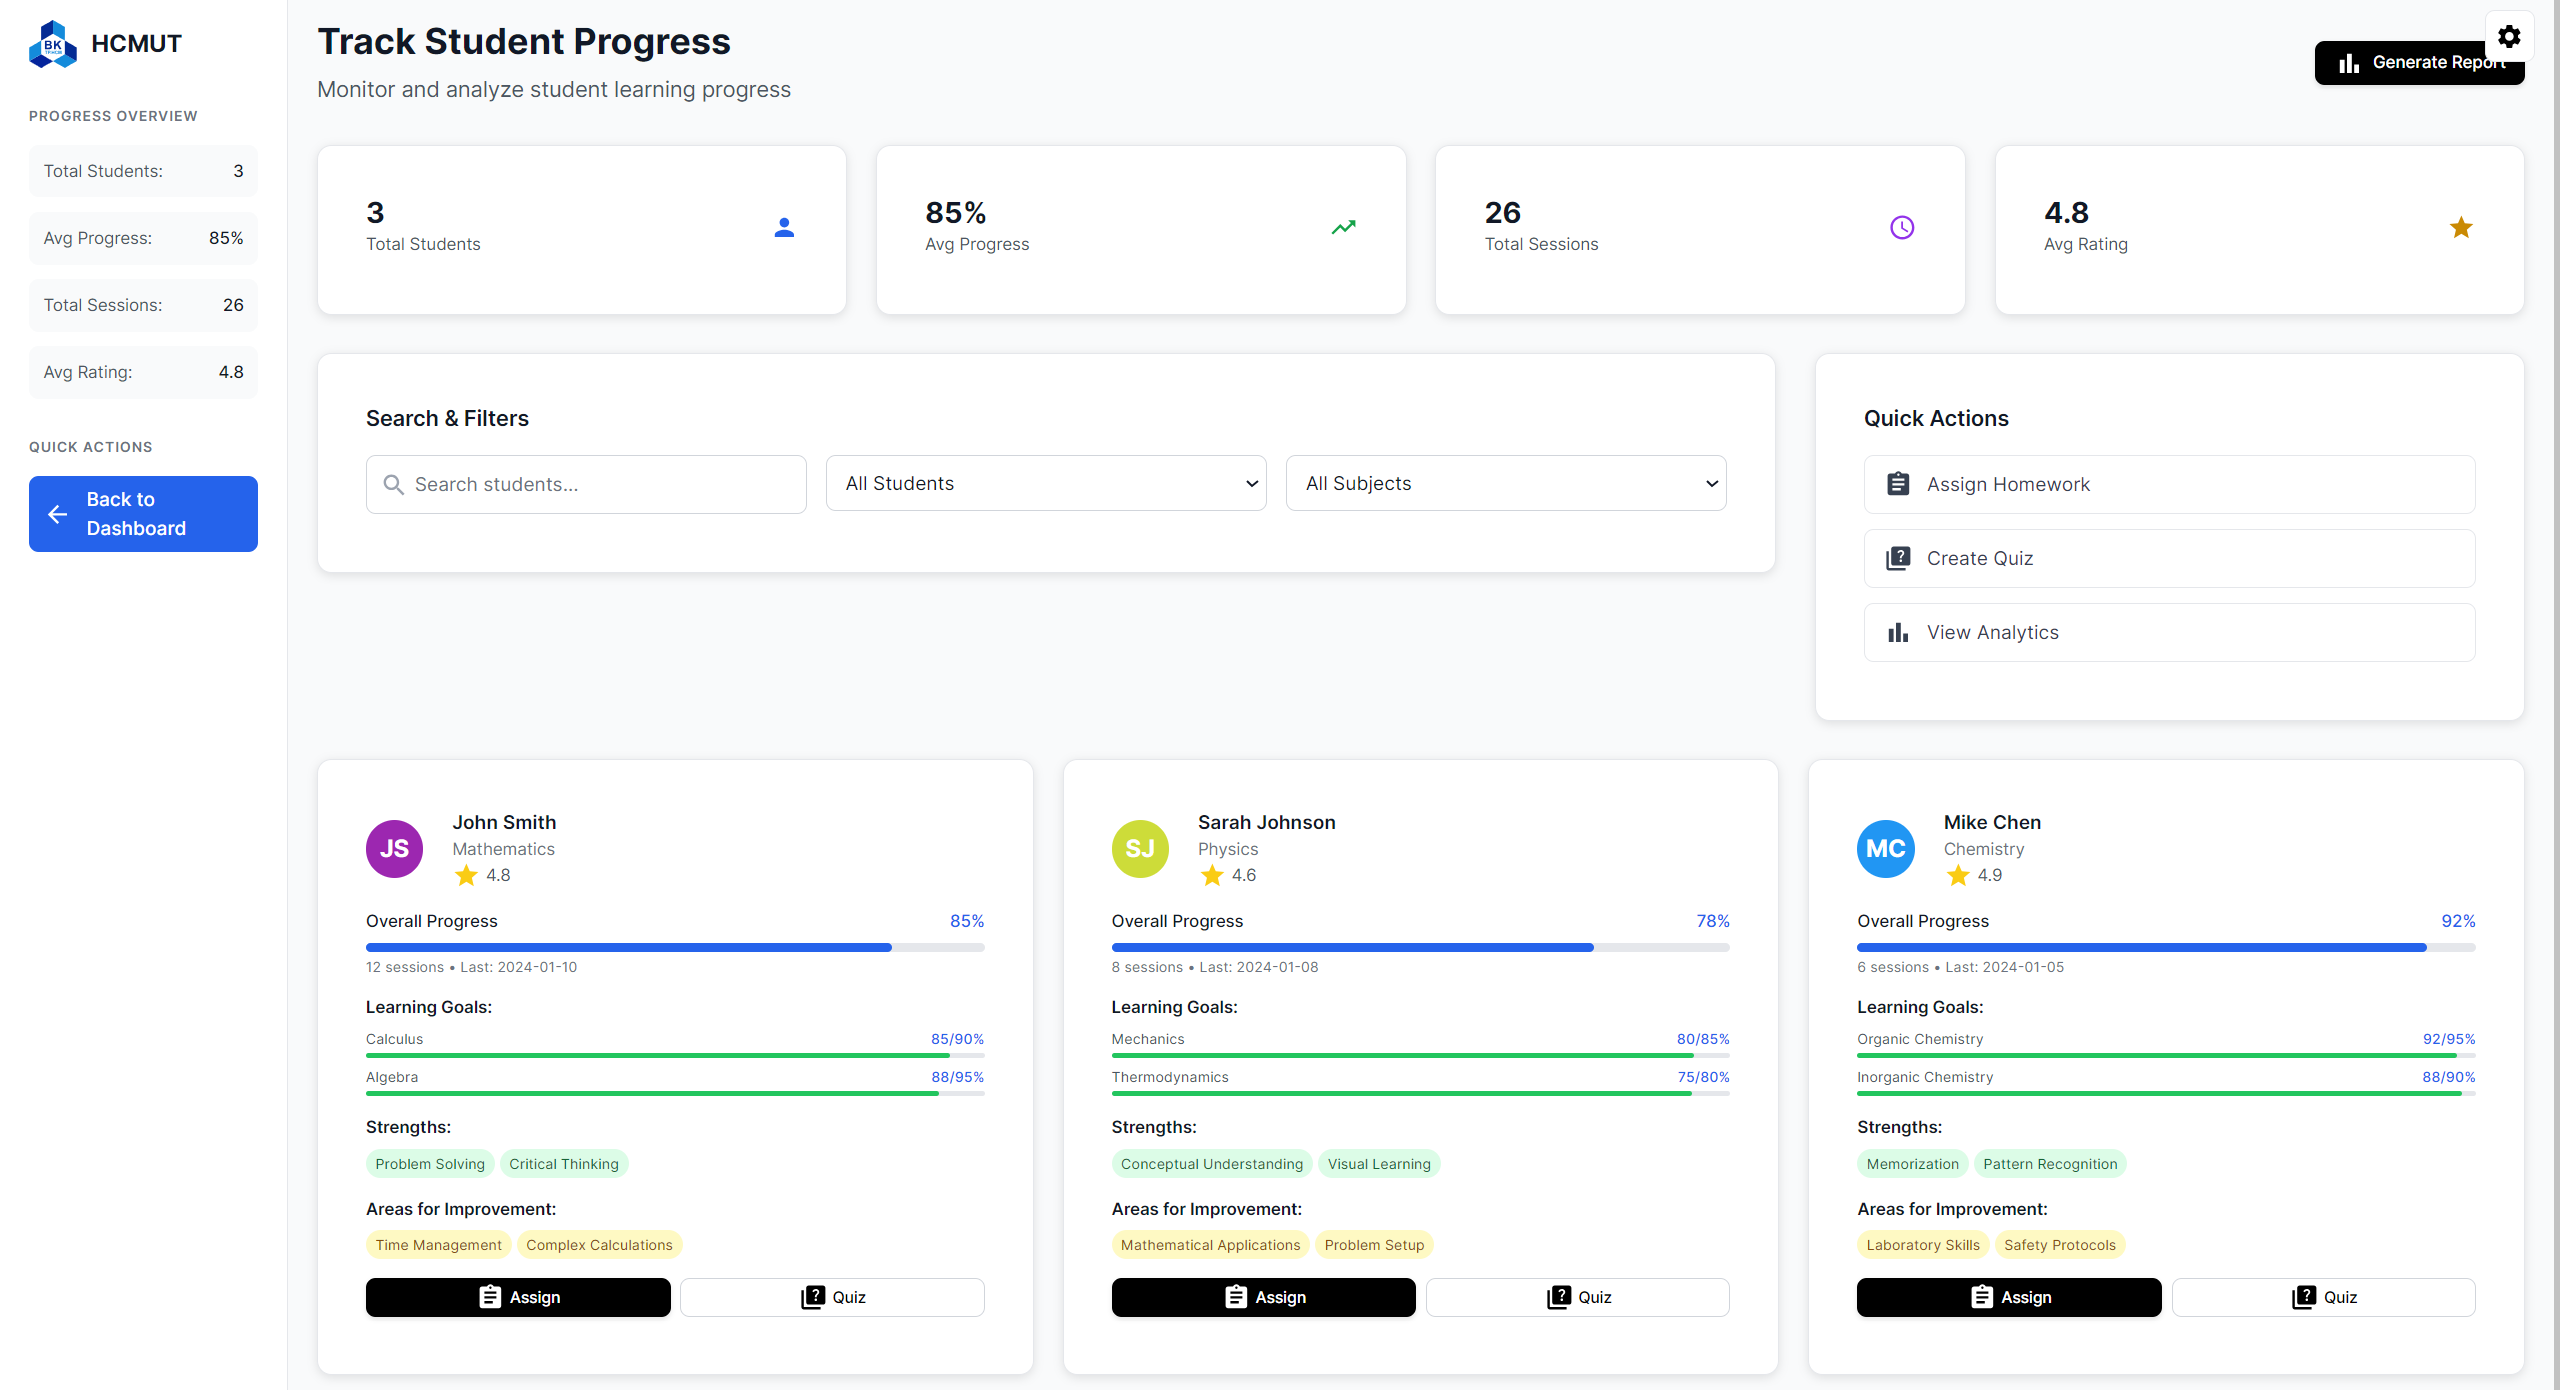
\includegraphics[width=\textwidth]{graphics/chapter2/tutor/track_student_progress_overall.png}
    \caption{Track Student Progress Page Overview}
    \label{fig:track_student_progress_overall}
\end{figure}

\paragraph{General Overview}
The page features a three-column layout with progress overview, summary statistics, search filters, and individual student progress cards.
